 \section{Inpainting}
 %MODIFIER ICI
 %%%%%%%%%%%%%%%
 % Frame Section title
 \begin{frame}
 \title{Inpainting}
 \titlepage

    \begin{minipage}{0.3\textwidth}
    \begin{flushleft} \large
    \emph{Binôme :}\\
    M. Keribin\\
    T. Rebele
    \end{flushleft}
    \end{minipage}
    \begin{minipage}{0.5\textwidth}
    \begin{flushright} \large
    \begin{figure}
    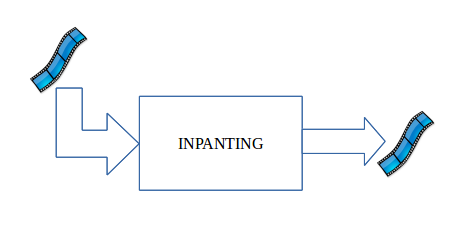
\includegraphics[width=1.4\textwidth]{Fig/architectureSectionInpainting.png}
    \end{figure}
    \end{flushright}
    \end{minipage}\\[3cm]
    
 \end{frame}



 %%%%%%%%%%%%%%%
 % Frame Architecture inpainting
\begin{frame}
  \frametitle{Architecture du programme}
  \insertF{Fig/architectureInpainting.png}{Architecture de la partie Inpainting}{1}

\end{frame}



 %%%%%%%%%%%%%%%
 % Frame KeyPoints
\subsection{Keypoints}
\begin{frame}
  \frametitle{Keypoints}
  
  \begin{itemize}
  \item SURF
  	\begin{itemize}
  	\item Inspiré des SIFTs
  	\item Plus rapide
  	\item Utilise ondelettes de Haar 2D
  	\end{itemize}
  	
  \item GFTT
    \begin{itemize}
    \item Utilise les points de Harris
    \item Détection de coins
    \end{itemize}
  	
  \item LucasKanade Optical Flow
    \begin{itemize}
    \item Grille sur chaque frame
    \item Suivi des keypoints dans la grille
    \item Adaptation du nombre de Keypoints
    \end{itemize}
  \end{itemize}
\end{frame}  	
  
\begin{frame}
  \frametitle{Keypoints}
  
  \begin{itemize}
  \item Canny : Détection des contours
    \begin{itemize}
  	\item Réduction du bruit
  	\item Gradient d'intensité
  	\item Détection des contours
  	\item Seuillage des contours
  	\end{itemize}
  	
  \end{itemize}
    \insertF{Fig/cannyPoints.png}{Points de Canny}{0.6}


\end{frame}



 %%%%%%%%%%%%%%%
 % Frame create trace
\subsection{Trace}
\begin{frame}
  \frametitle{Trace}
  \begin{itemize}
  \item Recherche de correspondances entre points
  	\begin{itemize}
  	\item Sélection des keypoints
  	\item Recherche dans le voisinage frame suivante
  	\end{itemize}
  \item Estimer l'homographie
  \item Trace
  	\begin{itemize}
  	\item Créer et continuer la trace
  	\item Classifier la trace
  	\begin{itemize}
  		\item fixe
  		\item mobile
  		\item indéterminé
  	\end{itemize}
  	\end{itemize}
  \end{itemize}
  
    \insertF{Fig/cannyKeypoints.png}{Mise en évidence des keypoints et de la trace}{0.4}


\end{frame}


 %%%%%%%%%%%%%%%
 % Frame inpainting principe
\subsection{Remplissage}
\begin{frame}
  \frametitle{Remplissage}
  
  \begin{itemize}
  \item Classifier les zones
  	\begin{itemize}
  	\item fixe $\leftrightarrow$ noir
  	\item mobile $\leftrightarrow$ couleur du fond
  	\end{itemize}
  \item Remplir quand le point devient fixe  
  \end{itemize}

  \begin{figure}
  
\includegraphics[width=0.33\textwidth]{Fig/bunny1-original.png}
  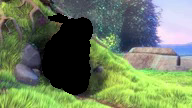
\includegraphics[width=0.33\textwidth]{Fig/bunny2-masked.png}
  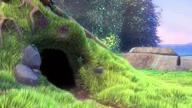
\includegraphics[width=0.33\textwidth]{Fig/bunny3-inpainted.png}
  \caption{Principe de l'inpainting 2D + t}
  \end{figure}
   
\end{frame}


 %%%%%%%%%%%%%%%
  % Frame demonstration
 \begin{frame}
   \frametitle{Démonstration}
   \begin{figure}
   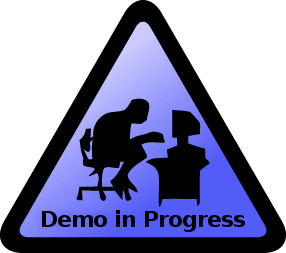
\includegraphics[width=0.5\textwidth]{Fig/demoInProgress.png}
   \end{figure}

 \end{frame}